\lstset {
	columns=flexible,
	tabsize=4
}

\section{Abstracción y modelado}
El objeto a modelar es una intersección de $N$ calles o avenidas. Con el objeto de profundizar el análisis, se tomará el caso de una intersección de dos avenidas, como la que se puede ver en la figura \ref{fig:interseccion-base}. A lo largo de este trabajo se utilizará el término \enquote{tramo} para designar al medio por el cual arriban vehículos o personas a la intersección. Una avenida de doble sentido de circulación tiene dos tramos. Con lo cual una intersección de dos avenidas tiene cuatro tramos más un tramo diferenciado para los peatones.

\begin{figure}[htbp]
	\centering
	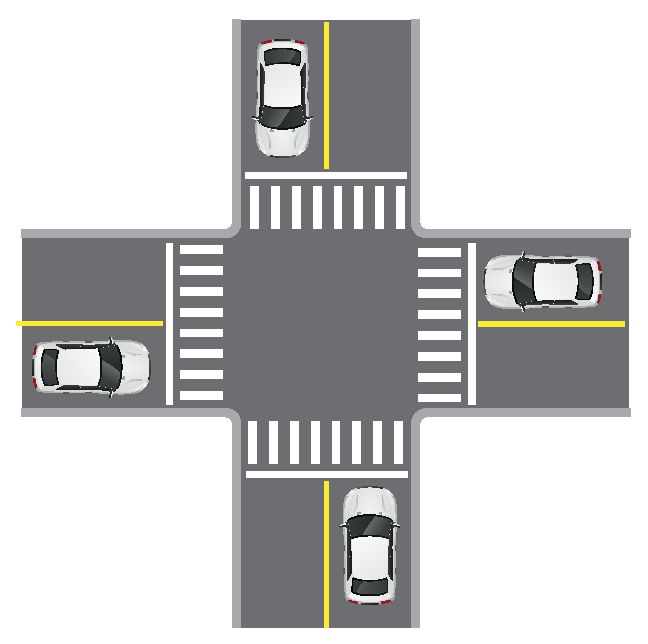
\includegraphics[width=6cm]{imagenes/interseccion-base.eps}
	\caption{Intersección base.}
	\label{fig:interseccion-base}
\end{figure}

Se asume que se existe una forma fiable de detectar la presencia de vehículos en un tramo. Se dice que un tramo está \enquote{activo} si y solo si hay al menos un vehículo en él.

Por otro lado, también se debe tener en cuenta la presencia de peatones. Para ello se asume que en cada senda peatonal de la intersección hay un pulsador que permite a un peatón solicitar el paso por una de las sendas peatonales. El tramo de peatones se activa con presionar una vez el pulsador y permanece activo hasta ser atendido. Se dice que un tramo es atendido cuando el sistema de semáforos permite el paso de vehículos o personas, es decir, tiene su semáforo correspondiente en verde.

Para simplificar el análisis, se modela a la intersección como un recurso compartido al cual se accede con exclusión mutua. Es decir, la intersección puede ser adquirida a lo sumo por un tramo.

\subsection{Especificación del comportamiento}\label{sec:spec}
Para entender mejor el problema a resolver se tuvo que analizar cada situación que se presenta en una intersección.
\subsection{Ningún tramo activo}
Cuando no hay ningún tramo activo, es decir, no hay vehículos en ninguna línea de detención, el sistema debe dar paso a todos los tramos de forma periódica y de a turnos (Round-Robin). Se puede ver esta situación en la figura \ref{fig:ningun-activo}.

Si estuviera activo el tramo del peatón, entonces se incluye al tramo de peatón al conjunto de tramos participantes del Round-Robin.

\begin{figure}[htbp]
	\centering
	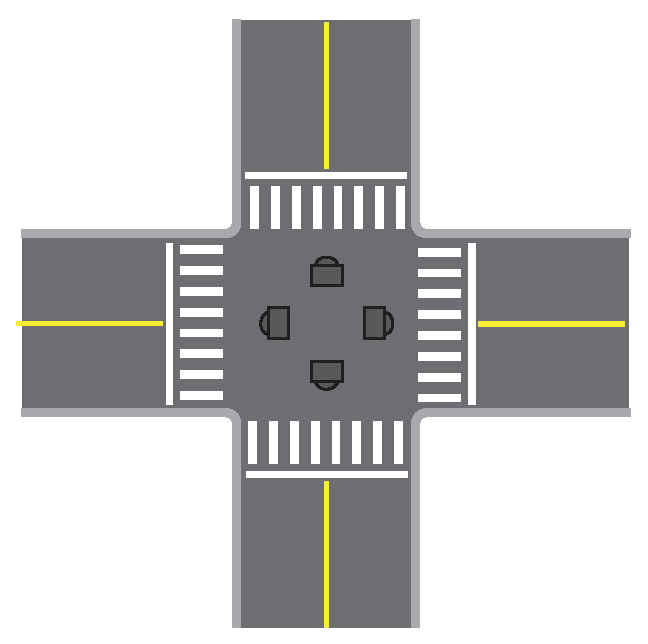
\includegraphics[width=6cm]{imagenes/ningun-activo.eps}
	\caption{Intersección sin vehículos ni peatón.}
	\label{fig:ningun-activo}
\end{figure}

\subsection{Un tramo activo}
Cuando hay un solo tramo activo, entonces se le debe dar el paso ininterrumpidamente hasta que haya otro tramo activo (esto incluye el caso en que se active el tramo de peatones).

Se puede ver la situación de estar un sólo tramo activo en la figura \ref{fig:un-activo}.

\begin{figure}[htbp]
	\centering
	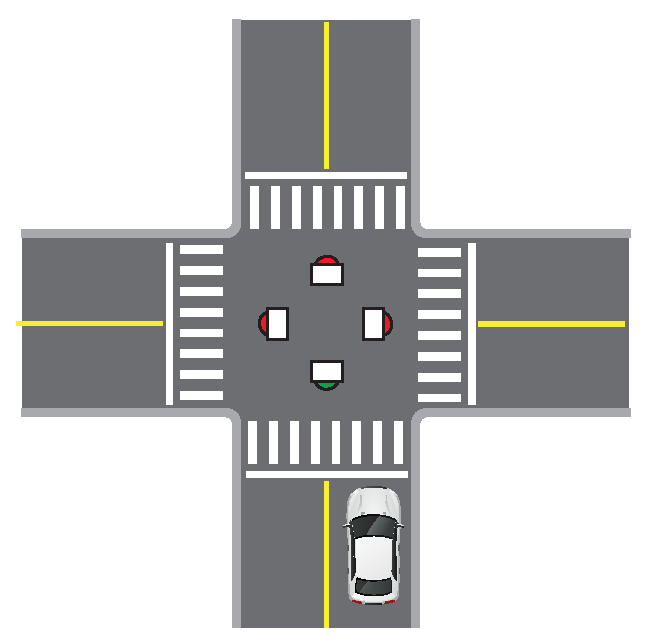
\includegraphics[width=6cm]{imagenes/un-activo.eps}
	\caption{Intersección con un tramo activo.}
	\label{fig:un-activo}
\end{figure}

\subsection{Más de un tramo activo}
Cuando hay mas de un tramo activo, simplemente debe hacerse Round-Robin como en el caso anterior pero sólo participan los semáforos correspondientes a los tramos activos, permanenciendo el resto en rojo.
\begin{figure}[htbp]
	\centering
	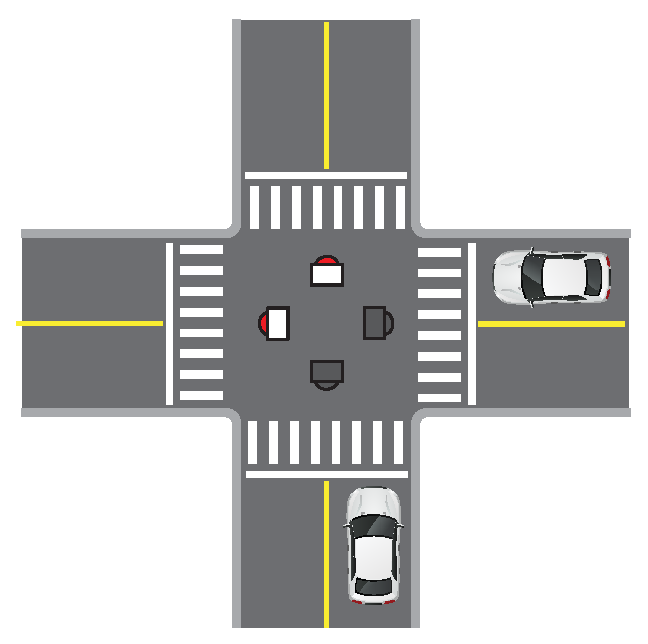
\includegraphics[width=6cm]{imagenes/dos-activos.eps}
	\caption{Intersección con dos tramos activos.}
	\label{fig:dos-activos}
\end{figure}

Se puede ver la situación de estar dos tramos activos en la figura \ref{fig:dos-activos}.

A modo de resumen, se lista las situaciones y el comportamiento correspondiente en la tabla \ref{tab:comportamiento}.

\rowcolors{2}{gray!25}{white}
\begin{table}[htbp]
	\centering
	\caption{Resumen de comportamiento del sistema ante distintas combinaciones de entrada.}
	\vspace{0.25cm}
	\label{tab:comportamiento}
	\begin{tabular}{cc}
		\toprule
		\bf{Tramos activos} & \bf{Comportamiento} \\
		\midrule
		0 & Round-robin entre todos los tramos. \\
		1 & Verde ininterrumpido al único tramo activo. \\
		$1 < \mbox{TA} \le N$ & Round-robin entre los tramos activos. \\
		$N$ & Round-robin entre todos los tramos activos. \\
		\bottomrule
	\end{tabular}
\end{table}

\subsection{Uso de procesos}\label{sec:proc}
Basándose en el marco teórico de la programación concurrente, se puede modelar a cada tramo como un proceso que trata de acceder al recurso compartido (la intersección). De esta forma el problema del control del tránsito se reduce al de la planificación de un recurso compartido. Este recurso compartido programáticamente se convierte entonces en una sección crítica.


\section{Implementación del sistema}
La implementación del controlador de semáforos se realizó sobre un Arduino Uno, utilizando la plataforma de desarrollo Arduino.Como herramienta de desarrollo se utilizó la extensión PlatformIO para el editor de texto Visual Studio Code.

FreeRTOS provee proyectos prearmados y preconfigurados para tomar como código base y realizar el desarrollo directamente sobre ellos. No existe una implementación oficialmente soportada por Real Engineers Ltd. (la empresa detrás de FreeRTOS), ni tampoco una implementación para el microcontrolador del Arduino Uno, el Atmega 328P. Sin embargo, existe una implementación no oficialmente soportada para Arduino Uno. El repositorio git de esta implementación está en \url{https://github.com/feilipu/Arduino\_FreeRTOS\_Library}.

Se realizaron tres implementaciones que implementan el sistema según lo especificado en la sección \ref{sec:spec}. Cada implementación hace uso de las distintas funcionalidades provistas por FreeRTOS de forma distinta, pero todas tienen en común el uso de semáforos, mútexes y tareas. Los procesos se traducen a tareas en FreeRTOS y la exclusión mutua perteneciente a la sección crítica mencionada en la sección \ref{sec:proc} se hace cumplir con el uso de semáforos y mútexes.

\section{Implementación A}
En esta implementación existe un controlador que controla que tareas (correspondiente a cada tramo) tiene que ejecutar en cada instante de tiempo.

El controlador realiza la planificación según los datos sensados de una clase sensor que lee la actividad de los tramos y se comunica mediante productor/consumidor para pasarle los datos al controlador.

El pseudo código de la tarea controlador se puede observar en el fragmento \ref{lst:imp-a}.
\begin{lstlisting}[label=lst:imp-a, caption=Pseudocódigo de la tarea controlador.]

while (true)
	Se sensa los tramos
	Si hay un tramo nuevo activo
		Se prende éste y se apaga el anterior en verde
		
\end{lstlisting}

Una de las desventajas es que se tiene muchas tareas en ejecución debido a que es necesario sensar constantemente los tramos y que se recurre a un controlador para la planificación

\section{Implementación B}
En esta implementación se trata de transferir hacia el kernel de FreeRTOS la responsabilidad de elegir cuál semáforo adquiere el recurso, es decir, a cual tramo se le da el paso.

Se tienen, al igual que en la implementación A, $N + 1$ ($N$ tramos y el tramo distinguido para los peatones) tareas, donde cada una representa un tramo y todas tratan de acceder a una sección crítica, protegida ahora por un sólo mútex.

Se utilizan dos valores de prioridad en las tareas, una alta y una baja. Las tareas correspondientes a tramos activos toman una prioridad alta y las tareas correspondientes a tramos inactivos toman una prioridad baja. La prioridad de las tareas está ligada a la actividad de su tramo, con lo cual las prioridades van variando a lo largo del funcionamiento del sistema.

Para que el orden en el cual cada tarea adquiere el mútex sea determinístico, no es suficiente que el planificador sea débilmente $fair$, sino que es necesario que se aplique una política de planificación que realice Round-Robin entre tareas de misma prioridad. FreeRTOS permite lograr esto mediante su archivo de configuración.

Cada tarea realiza el algoritmo explicitado en el código \ref{lst:imp-b}.

\begin{lstlisting}[label=lst:imp-b, caption=Pseudocódigo del programa que corre cada tarea en la implementación B.]
	while (true)
		P(mutex)
		do
			Verde()
			Delay(...)
			Leer sensores y actualizar prioridades
		while (Este tramo sea el unico activo)
		Amarillo()
		Delay(...)
		Rojo()
		Delay(...)
		V(mutex)
	Fin while
\end{lstlisting}

\section{Implementación C}

La tercera implementación de este proyecto surge con la necesidad de eliminar los problemas que se introducen en las anteriores soluciones.
El principal inconveniente que se busca solucionar, se relaciona con el uso de las proiridades dinámicas.
En particular, cuando se le cambia la prioridad a una tarea que se encuentra en el estado bloqueada, el programa no responde tal como era de esperarse.

Para esta implementación se sigue modelando a cada tramo como una tarea de FreeRTOS (incluyendo al de los peatones) y se toma las mejores características de los anteriores diseños.
En primer lugar, las prioridades vuelven a ser estáticas, evitando así el problema del cambio de prioridades sobre tareas que no se encuentren en estado Ready-To-Run ni Running.

Por otra parte, se elimina la existencia de un proceso controlador.
La tarea de planificación queda a cargo del kernel de FreeRTOS.
De esta forma el diseño de la solución queda más simple, tal como en la segunda implementación.
No se utilizan búffers, ni el modelo productor/consumidor y los recursos se aprovechan al máximo.

Es fácil de extender a más tramos, por ejemplo si se agrega el cruce con un diagonal.
Además permite pensar al peatón como un semáforo más, cosa que no ocurría en la primera implementación.

La principal diferencia respecto de las anteriores soluciones es que en este diseño, la intersección no se implementa con un único mútex.
Cabe destacar que se sigue pensando como una sóla sección crítica pero en su codificación representa un mútex por cada tarea.

De esta forma cada proceso se duerme en su propio mútex e independientemente de la actividad que haya en su tramo, se garantiza que en algún momento entra a la sección crítica.
Cuando dicho evento ocurre, la tarea tiene posibilidad de consultar con su sensor si hay autos o peatones (según corresponda) esperando por cruzar, y en caso afirmativo, coloca verde en su semáforo.

Al finalizar su trabajo, la tarea despierta a la próxima para que tenga posibilidad de ejecutarse, y la primera se vuelve a dormir en su propio mútex nuevamente hasta que le toque correr otra vez.

Este diseño permite que las tareas se autocontrolen sin la necesidad de la existencia de un proceso controlador.

Cada tarea realiza el algoritmo explicitado en el código \ref{lst:imp-c}.

\begin{lstlisting}[label=lst:imp-c, caption=Pseudocódigo del programa que corre cada tarea en la implementación C.]
	while (true)
		P(mutex[i])
		if (es activo o no hay activos)
			do
				Verde()
				Delay(...)
				Leer sensores
			while (Este tramo sea el unico activo)
			Amarillo()
			Delay(...)
			Rojo()
			Delay(...)
		V(mutex[i++])
	Fin while
\end{lstlisting}
